\documentclass{article}
\usepackage[utf8]{inputenc}
\usepackage[T1]{fontenc} 
\usepackage[french]{babel}
\usepackage{graphicx}
\usepackage{subfigure}
\usepackage[table]{xcolor}
\usepackage{geometry}
\usepackage{hyperref}
\usepackage{appendix}
\usepackage{pdfpages}

\geometry{hmargin=2.5cm,vmargin=3cm}
\setlength{\parskip}{0.1cm}

\title{Rapport de Stage}
\author{Laureline MARTIN}
\date{Mercredi 7 Octobre 2020}

\begin{document}
\maketitle
\vspace*{14cm}
\begin{center}
	\textbf{Encadrants :}
\end{center}
\begin{tabular}{p{4cm}p{4cm}p{8cm}}
	\hspace*{-1cm}
	Mme. Viviane GAL & Ingénieure & Equipe \textit{Interactivité pour lire et jouer - ILJ}\smallskip\\
	\hspace*{-1cm}
	M. Eric GRESSIER-SOUDAN & Professeur des universités & Equipe \textit{Réseaux et Objets Connectés - ROC}
	\smallskip\\
	\hspace*{-1cm}
	Mme. Elena KORNYSHOVA & Maître de conférences & Equipe \textit{Igénieurie des systèmes d'information et de décision - ISID}
\end{tabular}


\newpage
\begin{center}
	\textbf{Résumé :}
\end{center}
\hspace*{0.4cm}
Durant cinq mois et demi, j'ai travaillé au laboratoire de recherche CEDRIC au Conservatoire National des Arts et Métiers de Paris.\par
Ce stage s'est inscrit au sein du projet exploratoire "Conception et développement des jeux pervasifs adaptables avec la prise en compte des états émotionnels des joueurs" du laboratoire.
L'objectif global de ce projet est de proposer un jeu pervasif où le joueur et ses émotions sont au coeur même du jeu. 
Pour cela, des capteurs physilogiques sont utilisés pour détecter et reconnaître les états émotionnels du joueurs ainsi que des capteurs placés dans l'environnement pour connaître le contexte global. 
Un état de l'art ainsi qu'une première version d'une ontologie afin de répondre à cet objectif ont été proposées et se trouvent dans ce rapport. 
Une solution pouvant lire les données provenant de capteurs physilogiques a également été proposée.
Cette solution envoie ces données à des algorithmes déjà existant qui permettent de traiter ces données pour en déduire des états émotionnels.
\bigskip\newline
\begin{center}
	\textbf{Abstract :}
\end{center}
\hspace*{0.4cm}
I worked for the CEDRIC research laboratory based on Conservatoire Nationnal des Arts et Métiers at Paris during five mounths and half.\par
This work was for the laboratory's exploratory project "Desing and development of adaptables pervasives games to players' emotional states".
The main project goal is to propose a pervasive game where player and his emotions are the heart of the game.
To reach this goal, physiological sensors are used in order to detect and recognize player's emotional states and others sensors are placed in environment to know the global context.
This report contains a state of the art and a first version of an ontology that I made. 
It contains a solution to read physiological sensors' data too.
This solution sends data to existing detection and recognition of emotional states algorithms.
\vspace*{4cm}
\begin{center}
	\textbf{Avant-propos}
\end{center}
\hspace*{0.4cm}
Dans le cadre de la validation du Master 2 Data Managment in a Digital World - Datascale, proposé par l'Université de Versailles Saint-Quentin / Paris Saclay, j'ai effectué un stage de cinq mois et demi du 16 Mars 2020 au 30 Septembre 2020.
Le contexte particulier lié à la crise sanitaire m'a amené à travailler pour la majorité de mon stage en télétravail (du 16 Mars au 10 Septembre).\par
Pour communiquer pendant cette période de travail à distance, nous utilisions les mails et nous avons organisé des réunions via Teams tous les 7 à 15 jours.
Ces réunions duraient entre une demie heure et une heure.
Ces sessions vidéos étaient l'occasion de faire le point sur l'avancement de mon travail et sur les tâches des jours à venir.
Cependant, la barrière de l'écran a créé un réel manque de spontanéité lors de nos échanges.
Pour ma part, je pense que les visio-conférences n'ont pas suffit pour échanger tout au long de cette période de télétravail. 
Peut-être qu'une autre forme de communication, comme une messagerie instantanée, ajoutée à celle des réunions sur Teams, aurait pu réduire se manque de spontanéité.\par
A l'issue de ce stage, je pense que les réunions en présentiel restent la meilleure manière de communiquer et de partager autour d'un projet.

\newpage
\renewcommand{\contentsname}{Table des matières}\tableofcontents

\newpage
\section{Introduction}
	Depuis plusieurs années, les jeux pervasifs se multiplient sur le marché, proposant aux joueurs des conetnus très immersifs.
	Le jeu pervasif (aussi appelé jeu omniprésent) est un genre de jeu qui mêle le monde physique et le monde numérique et rend floue cette frontière.
	% Comme le décrit Astic dans \cite{astic_2013},
	Dans le jeu pervasif, le contexte est essentiel. 
	Quatre facteurs sont mis en jeu : l'espace, le temps, la technologie et les rapports sociaux. 
	L'espace du jeu pervasif est à la fois ancré dans le réel et à la fois virtuel.
	Il convient alors que des ponts existent entre ces deux espaces. 
	Ces ponts peuvnet se faire via des objets, des points géographiques, des personnes, etc. 
	Le temps est calqué sur le temps réel mais il peut être utilisé de différentes manières. 
	L'heure et/ou le jour peuvent influencer le comportement que doit adopter le joueur.
	La technologie est également importante. 
	Elle doit rester accessible au joueur, tant sur le plan pratique que sur le plan financier. 
	La géolocalisation, les réseaux sans fil, etc. sont des technologies utilisées pour ce type de jeu.
	Dans les jeux pervasifs, les joueurs, les spectateurs et les non-joueurs sont mélangés sur le même espace. 
	Les joueurs n'ont pas de caractéristiques particulières pour se reconnaître.%\par
	Le jeu pervasif à un un impact social et culturel important.
	Il favorise les récontres dans l'espace physique.
	Il permet de découvrir de nouveaux endroits, de nouvelles choses et de s'enrichir culturellement.
	Cependant, le jeu omniprésent ne met pas réellement le joueur au centre de jeu.\par
	Le projet "" vise à meettre le joueur et ces émotions au centre du jeu.
	C'est les émotions du joueurs qui influenceront les événements du jeu.
	Pour pouvoir détecter et reconnaître les ététs émotionnels du joueur afin que le jeu s'y adapter et propose l'événement le plus adéquant, de multiples capteurs physiologiques doivent être utilisés.
	Ces capteurs généèrent beaucoup de données qui doivent stockées et traités.
	Ces données permettront à des a des algorithmes de reconnaître les états émotionnels.\par
	Le but de ce travail a été de dresser le contour et d'affiner le conceptualisation d'un jeu pervasif adaptable aux états émotionnels du joueur. 
	Dans ce rapport, nous nous sommes intéressés, d'une part, à l'adaptation de jeu selon le contexte émotionnel et d'autre part, à la gestion de données générées par les capteurs physiologiques.\par
	Nous allons tout d'abord présenter l'état de l'art présentant différentes approches pour l'adaptation dynamique d'un jeu pervasif aux états émotionnels du joueur.
	Nous aborderons l'expérience que nous avons mené lors d'un escape game et la notion d'expérience .
	Puis nous présenterons une ontologie non-aboutie d'un jeu pervasif prenant en compte l'état émotionnel du joueur.
	Enfin nous présenterons une solution pour la gestion de données provenant de capteurs physiologiques

	J'ai rejoins ce projet à son commencement. 
	Le but de mon stage est double : 
	d'une part, je dois recueillir et synthétiser les éléments déjà existants dans la littérature scientifique et industrielle pour l'élaboration d'un tel jeu pervasif. 
	Et d'autre part, je dois élaborer un modèle conceptuel afin de représenter les éléments qui permettront par la suite d'implémenter ce jeu particularisé.\par
	Dans ce rapport, je vais tout d'abord présenter le laboratoire ainsi que l'équipe avec laquelle j'ai travaillé et son projet. Puis, je présenterai ...

\section{Le projet}
	Le projet exploratoire initié par trois enseignants-chercheurs du laboratoire CEDRIC du CNAM de intitulé "Conception et développement des jeux pervasifs adaptables avec la prise en compte des états émotionnels des joueurs" vise à élaborer un jeu pervasif capable de s'adapter dynamiquement selon le contexte du joueur et son environnement.\par
	Le but est de concevoir un jeu omniprésent capable de détecter et de reconnaître dynamiquement l'état émotionnel courant de joueur. 
	Il faut aussi que le jeu puisse s'adapter à cet état en temps réel en proposant un événement spécifique. 
	Cet événement devra soit maintenir le joueur dans l'état émotionnel courant, soit changer l'état émotionnel du joueur. 
	Le choix de maintenir ou de changer l'état émotionnel du joueur devra se faire par rapport au context environnemental.
	Cependant, la conception d'un tel jeu doit rester assez générique pour pouvoir l'appliquer à d'autres domaines dans de prochains projets.\par 



\section{Cadre du stage}
	\subsection{Le laboratoire CEDRIC}
		\begin{center}
			
\includegraphics[scale=0.45]{../include/logo-cedric.PNG}\\
		\end{center}
		\hspace*{0.4cm}
		Pour ce stage, j'ai été accueillie par le laboratoire de Centre d'Etudes et De Recherche en Informatique et Communication (CEDRIC)\footnote{\href{http://cedric.cnam.fr/lab/accueil/labo/}{http://cedric.cnam.fr/lab/accueil/labo/}} au sein du Conservatoire National des Arts et Métiers (CNAM) de Paris\footnote{\href{http://www.cnam.fr/portail/accueil-conservatoire-national-des-arts-et-metiers-821166.kjsp}{http://www.cnam.fr/portail/accueil-conservatoire-national-des-arts-et-metiers-821166.kjsp}}. 
		Le laboratoire se situe au 2 rue Conte 75003 PARIS.\par
		Le laboratoire CEDRIC est composé de huit équipes ayant des actions dans le domaine de l'informatique fondamentale et appliquée, ainsi que dans d'autres disciplines proches (statistiques, électronique,...).
		\begin{itemize}
			\item L'équipe Données complexes, apprentissage et représentations (Vertigo) : Extraire de l'information et construire des méthodes de gestion de données basées sur le contenu pour des données massives audios, images et vidéos;
			\item L'équipe Interactivité pour Lire et Jouer (ILJ) : Questions autour de l'interaction homme-machine concernant des activités telles que le jeu et la lecteure. Cette équipe mèle plusieurs disciplines (informatiques, psychologie, design, arts,...) afin de répondre aux études en cours qui concernent la modélisation de la difficulté dans les jeux, les méthodologies de game design inclusif,...;
			\item L'équipe Ingénieries des Systèmes d'Information et de Décision (ISID) : Réunie autour de trois axes de recherche (les systèmes décisionnels, le web sémantique et la qualité des systèmes d'information) dans le but de concevoir des méthodes, des outils et des techniques	pour la conception et l'analyse de systèmes d'information et de décision dans tous les domaines;
			\item L'équipe Traitement du signal et architectures électroniques (LAETITIA) : Concentrée sur trois axes de recherhe : traitement du signal pour les télécommunications (recherches en lien avec les réseaux cellulaires (5G/6G) et en lien avec les problématiques de couches physique pour les réseaux faible puissance longue portée pour l'IoT), sûreté de fonctionnement des sytèmes dynémiques (recherche en automatique) et implémentation temps-réel (mise en oeuvre des algorithmes proposés par l'équipe);
			\item L'équipe Méthode Statistique de Data-Mining et Apprentissage (MSDMA) : Traitement de données et développement de modèles d'apprentissage statistiques dans le but d'extraire des information pour prise de décision;
			\item L'équipe Optimisation Combinatoire (OC) : Rassemblée autour de deux axes : la programmation mathématique et applications ainsi que les graphes et optimisation;
			\item L'équipe Réseaux et Objets Connectés (ROC) : Porte sur l'analyse et l'exploitation des nouvelles architectures réseaux et des systèmes liés à la virtualisation, à la mobilité et au développemnt des objets connectés;
			\item L'équipe Systèmes Sûrs (SYS) : Spécialisation, conception, vérification et évaluation des systèmes. Pour cela, Les recherches se font autour de trois axes : l'axe typage, sémantique et preuve, l'axe architecture logiciel, architecture systèmes et ligne de produit et l'axe vérification  et évaluation de systèmes parallèles et asynchrones.
		\end{itemize}
	\subsection{L'équipe}
		L'équipe de recherche est constituée de trois enseignants-chercheurs du CNAM travaillant dans trois équipes différentes :
		\begin{itemize}
			\item Mme Elena KORNYSHOVA, Maître de conférences travaillant au sein de l'équipe \textit{Igénieurie des systèmes d'information et de décision - ISID}, 
			\item Mme Viviane GAL, ingénieure travaillant au sein de l'équipe \textit{Interactivité pour lire et jouer - ILJ},
			\item M Eric GRESSIER-SOUDAN, professeur des universités travaillant au sein de l'équipe \textit{Réseaux et Objets Connectés - ROC}
		\end{itemize}
		Tous m'ont encadré tout au long de mon stage.

\section{Cadre du projet}
	Le projet "Conception et développement des jeux pervasifs adaptables avec la prise en compte des états émotionnels des joueurs" est un projet exploratoire du laboratoire CEDRIC.
	\subsection{Motivation et objectif}
		L'objectif gloabl de ce projet est de proposer une expérience de jeu pervasif unique où le joueur et ses émotions seraient au coeur du jeu. 
		Pour cela, le jeu doit pouvoir s'adapter au joueur en fonction du contexte global. 
		C'est-à-dire que le jeu doit pouvoir détecter et reconnaître l'état émotionnel courant du joueur,
		Il doit également pouvoir proposer l'événement le plus adapter en réponse à cet état émotionnel.\par
		Dans un premier temps, le but de ce projet est de formuler un modèle conceptuel du jeu pervasif adaptatif et dynamique basé sur les états émotionnels et sur le contexte environnent. 
		Et dans un second temps, de développer une approche d'ingénerie situationnelle du système d'information pour ce type de jeu tout en restant générique pour des applications à de multiples domaines.
	\subsection{Problématique}
		L'adaptation aux émotions est un problème complexe à différents niveaux.
		Il faut tout d'abord pouvoir détecter la présence d'un état émotionnel.
		Déjà plusieurs questions ce poses comme par exemble quel outil utilisé pour la détection ?\par
		Une fois détecter, il faut pouvoir reconnaître l'état émotionnel. Quelle approche utilisée ? Quel algorithme ? Pour quel(s) état(s) ?\par
		Une fois que nous connaissons l'état émotionnel du joueur, il faut pouvoir lui proposer un événement adapté à cet état. Plusieurs problèmes se posent, faut-il proposer un événement allant dans le sens de l'état émotionnel actuel du joueur ? Ou au contraire, lui proposer un événement susptible de changer son étaté émotionnel ? Quels événements sont attachés à quels états émotionnels ?\par
		De plus, tout cela doit pouvoir se faire en temps réel pour éviter un effet de décalage entre le joueur et le jeu qui pourrait distraire le joueur et le désintéressé du jeu.\par

\section{Etat de l'art}
	\textit{Voir Annexe \ref{ann:eda}.}

\section{Utilisation des données physiologiques}
	\subsection{Capteurs}
	\subsection{Middleware Oriented Messages (MOM)}
		\subsection{Comparaison entre Apache Kafka et RabbitMQ}
		\subsection{Choix de Apache Kafka}
	\subsection{Prototype : utilisation de Kafka pour des données physiologiques}

\section{Conclusion}




\newpage
\appendix
\section{Annexe 1 : Offre de stage}\label{app:annexe1}
	\textbf{Elaboration du modèle conceptuel des jeux pervasifs adaptables avec la prise en compte des états émotionnels des joueurs}\par
	\medskip
	\textbf{Contexte :}\newline
	Le champ des jeux affectifs est nouveau. Il s’appuie sur l’intégration de nouveaux moyens à développer dans les jeux afin d’adaptabilité. [1] et [2] présentent une méthodologie unifiée pour la conception des jeux affectifs utilisant le plus tôt possible le mécanisme de boucle émotionnelle. Ils repèrent des variations à l’aide de mesures physiologiques et appliquent un modèle issu d’un ensemble construit considéré comme en relation avec les émotions. Leur étude montre combien la dimension émotionnelle de l’utilisateur est importante mais difficile à gérer.\newline
	Le profil du joueur, y compris ses émotions, impacte la conception des jeux. Afin de proposer une meilleure expérience aux joueurs et de proposer un jeu particularisé, le jeu doit être adaptable en fonction du contexte global du joueur. Nous sommes dans une approche holistique qui combine à la fois l’individu et ses émotions, et, les influences de l’entourage qui va du bâtiment lui-même à l’atmosphère que dégage le lieu. Très peu de travaux ont été faits pour la conception et le développement des jeux adaptables dynamiquement. [3] formalise le concept des jeux appliqués aux visites de musées. Ce travail modélise le jeu de visite et propose un processus d’équilibrage entre la dimension ludique et la dimension non ludique (la visite) de ce type de jeux. [3] propose des patrons de mission qui servent d’éléments réutilisables lors de la conception des jeux, mais qui ne couvrent qu’une partie du processus de conception.\par
	\textbf{Sujet :}\newline
	Il s’agit dans ce stage d’élaborer un modèle conceptuel du jeu pervasif adaptable basé sur les émotions. Ce modèle, éventuellement réalisé sous forme d’une ontologie, doit couvrir toute la variété des facteurs qui impactent le jeu tels que le profil de l’utilisateur et ses données physiologiques exprimant son état émotionnel. Cette ontologie doit être construite de façon à ce qu’elle soit adaptée à la démarche situationnelle nécessaire pour la composition dynamique du jeu.

\section{Annexe 2 - Adaptation d’un jeu pervasif particularisé basée sur l'état émotionnel et sur les caractéristiques du joueur – État de l’art}\label{ann:eda}
	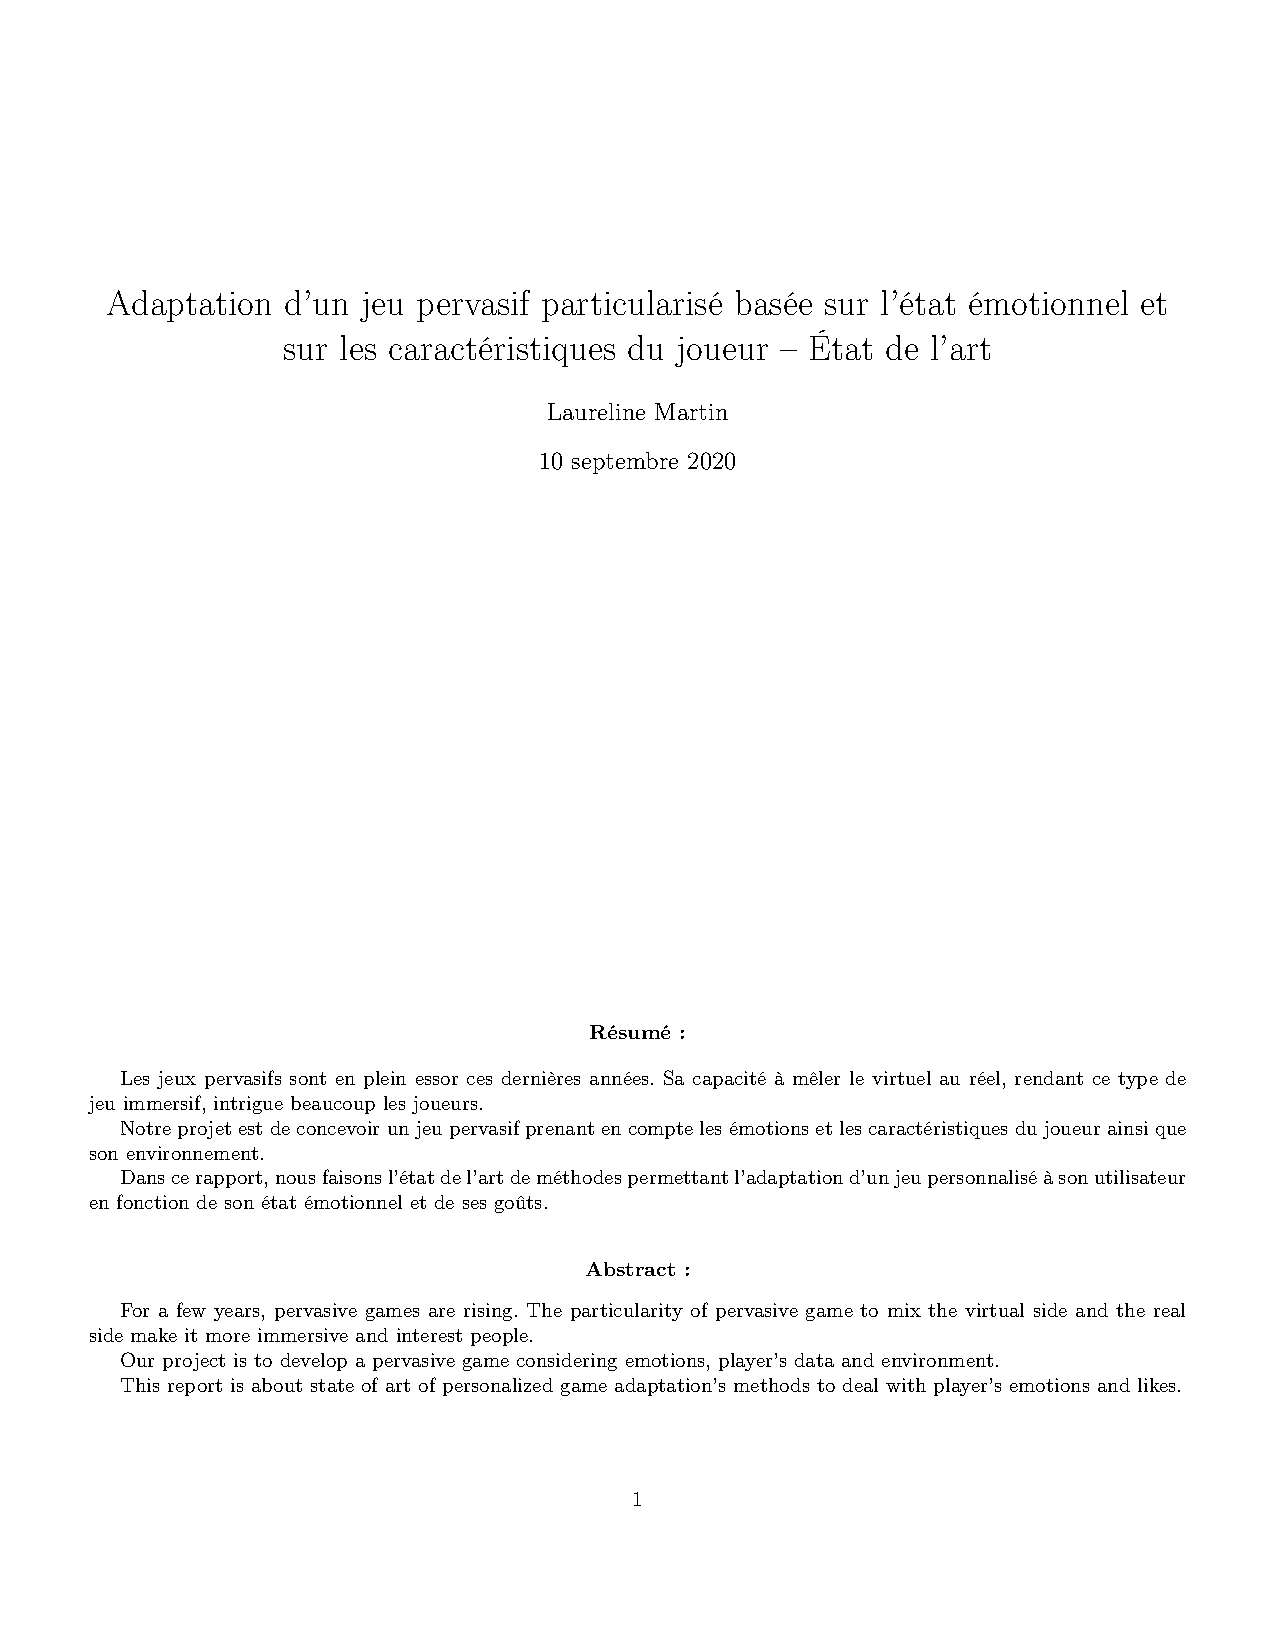
\includepdf[pages=-]{../include/eda.pdf}

%\section{Annexe 3 - Les classes en détail}\label{ann:detailclasse}
%	\includepdf[pages=-]{../include/classes.pdf}

%\section{Annexe 4 - Synthèse comparative entre Kafka et RabbitMQ}%\label{ann:kafkarabbitmq}
%	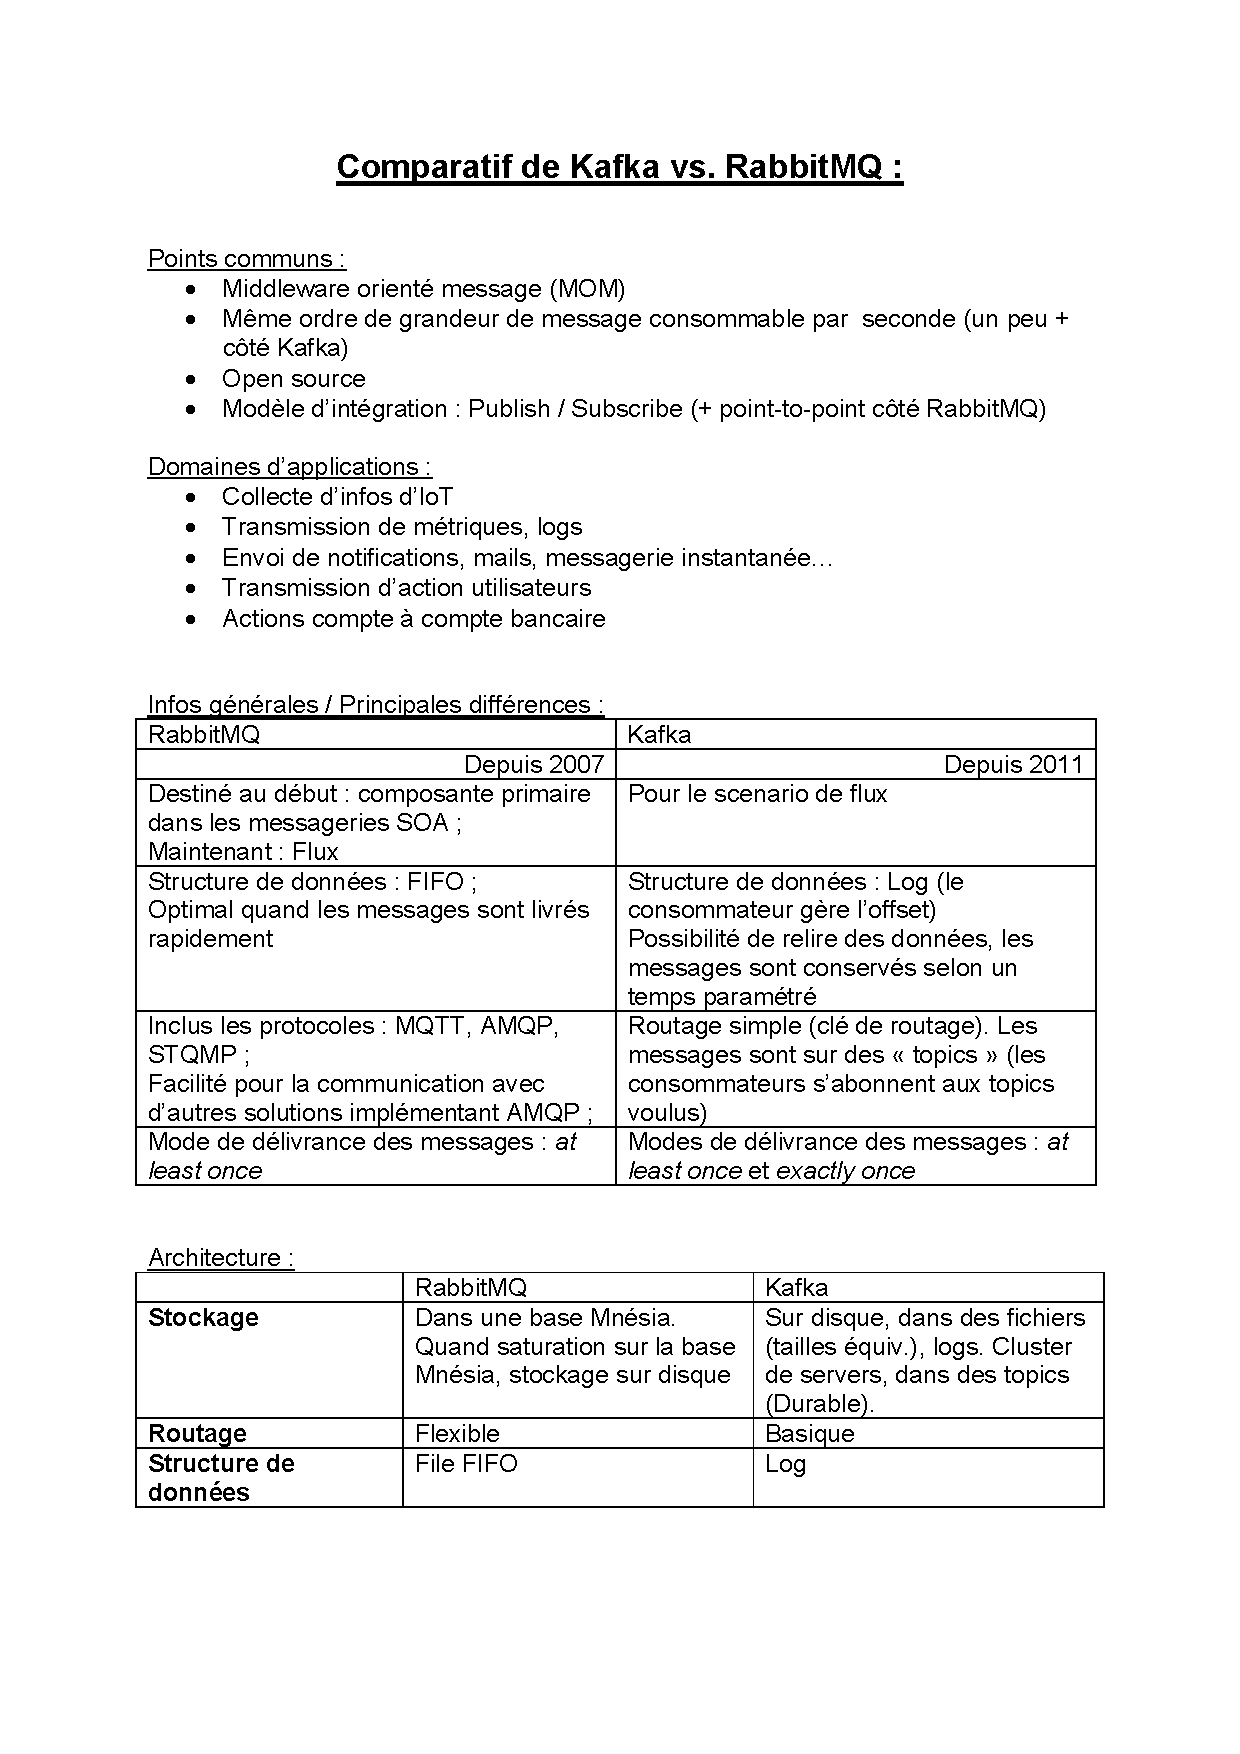
\includepdf[pages=-]{../include/comparatifKafkaVSRabbitMQ.pdf}	

\bibliographystyle{abbrv}
\bibliography{../include/biblio}
\end{document}